\documentclass{article}
\usepackage[utf8]{inputenc}
\usepackage[section]{placeins}

\title{NO-DOUBT: A Decision Support Web Platform based on AHP}
\author{Georgia Dede, Dimitrios Alexandrakis, Ioannis Nikolaou, Thomas Kamalakis}
\date{Harokopio University of Athens, Department of Informatics and Telematics}


\usepackage{natbib}
\usepackage{graphicx}

\begin{document}

\maketitle



\section*{Summary}
The DecisiOn sUpport weB plaTform (NO-DOUBT) aims to assist in complicated multicriteria decision making problems, using the Analytic Hierarchy Process (AHP). The AHP has been used around the world in a wide variety of decision situations, in fields such as government, business, industry,healthcare, education, project management \citep{chan2006ahp},\citep{dede2010evaluation},\citep{drake1998using},\citep{lee2006investigating},\citep{liberatore2008analytic},\citep{saaty2003decision}.

This application, extensively uses algorithms in order to solve a multicriteria problem, calculating weights for each criterion, factors (sub-criteria) that characterize the criteria, and the alternative solutions of a target. This online application was implemented by using PHP and HTML, an SQL database and Lapack libraries \citep{Lapack}, which are used to calculate eigenvalues and eigenvectors that help evaluating the weights for each criteria, factors and alternatives.

The NO-DOUBT tool offers a web based interface in order to create a survey, to determine a group of users who participate in the survey, to collect responses, and export results. In this context, this platform not only supports the AHP methodology but also the user administration, the surveys development, the definition of decision making problems. Each user has the opportunity to participate in a survey and view the results of previous surveys. Towards this end, there are two different interfaces, these of administrator and user with separate functionalities. The tool's implementation demonstrates the convenience that a decision maker can conduct a survey through a decision-making service, using simple data forms and programming structures. Furthermore, through this service, materialized algorithms of decision-making based on AHP are provided, in order to help finding the optimal solution in a rapid and easy way.

This tool is a web based supporting tool for decision making that can be helpful both for daily simple
decision problems and complex decision making problems in every day life, organizations, academia and industries.

\section*{Statement of Need}
Inspection of previous efforts reveals that there is a variety of tools that support the AHP methodology either commercial or open source (OSS). 

For example, super decisions software \citep{Superdecisions} is a free educational software. It is the only free educational software that implements AHP and was developed by the team of the creator of the method, Thomas Saaty. Its development and maintenance is sponsored by Creative Decisions Foundation.
Moreover, the expert choice \citep{Expertchoice} combine collaborative team tools and proven mathematical techniques based on decision making methods such as the AHP. 
The concluder \citep{Concluder} is a simple tool for complex decision making using the consistency-driven pairwise comparisons method (CDPC) which is primarily for multi-criteria decision making, such as the AHP. 
The AHP-software \citep{AHP-Software} is also used to solve the AHP in decision making and operation research. The spicelogic AHP Software \citep{AHP_Software}  captures the AHP methodology

Furthermore, open source software have been also developed for the AHP. More specifically,  the AHP-OS \citep{AHP-OS} is a free web based AHP tool for decision making processes. 
The AHP with R \citep{AHP-R} is an R package to model complex decision making problems using AHP. There are also other efforts that suppoty part or the whole AHP algorithm such as  \citep{Paulgovan}, \citep{Andrugo}, \citep{Airiyu}, \citep{Humberoroa}, \citep{Pvlhx}, \citep{Hogivano}. 

Even though there are several software that support AHP there is no single solution that offers a web based platform which both administrator and user functionalities. Most of the already developed AHP software integrate only the AHP algorithm. The NO-DOUBT tool supports the development of surveys, the management of users (registration, login) as well as the application of the AHP algorithm with extraction functionalities for further use of the results. There are many directions for future expansion of this tool. Towards this end, the authors have already begun to incorporate their research contributions in the field of decision making and more specifically, the estimation of the probability of rank reversal in order to investigate the stability of the final outcomes\citep{dede2015convergence},\citep{dede2016theoretical}.

\section*{AHP Methodology}
AHP is a multi-criteria decision making methodology which adopts a hierarchical form using three conceptual levels. In the first level, the objective is defined (e.g. the evaluation of technologies for home networking based on a set of alternative solutions). In the next level, we identify a number of criteria $N$ on which our evaluation will be based. Each criterion $C_k$ is an important aspect of the decision making problem and is further identified by its factors at the third level of the hierarchy. A factor $F_{j_k}$ is an indicative attribute that characterizes a criterion (e.g., downstream throughput is a factor of performance criterion for home networking technologies). 

In order to rate the alternative solutions, one must first evaluate the weights of the criteria $w_k$ and the factors $f_{j_k}$. Toward this end, each expert $m$ performs a series of PWCs by filling out a table containing the upper triangular elements based on a certain scale (e.g. the nine level scale). The diagonal elements of the PWC are set equal to one, while the lower triangular elements are calculated as the reciprocal of the upper ones.

The criteria weights for the $m$ expert are obtained by the elements of the eigenvector corresponding to the maximum eigenvalue of the PWC matrix. 

A similar procedure is followed for the estimation of the weights of the factors $f_{jk}$ of each criterion. Finally, the alternatives are pairwise compared according to each factor and for each alternative $A_i$ one obtains the relative scores $S_{ijk}$ under factor $F_{jk}$. The final ranking priorities $T_i$ of each alternative are evaluated by multiplying the relative scores $S_{ijk}$ by the overall weight $f_{j_k} · w_k$ of the corresponding factor as follows:

\begin{equation}
    T_i=\sum_{k=1}^{N}\sum_{j=1}^{J_k}S_{ijk} f_{jk} w_k
\end{equation}

\section*{Functionalities}
The NO-DOUBT tool is user friendly with clear and easy to follow procedures. The site is separated by user and administrator accounts. 
The administrator can create, modify and delete surveys, assign users to answer a survey and extract research results based on the user answers. On the other hand a user can register and answer an assigned survey as well as view his judgments and results.


\subsection*{Administrator}

The administrator can find all the possible actions in a sidebar in his main screen as presented below:

\begin{figure}[h!]
\centering

\includegraphics[scale=0.2]{admin_main}
\caption{Admin Main Page}
\label{fig:admin_main}
\end{figure}


\subsubsection*{Creating a Survey}

The administrator will have to complete a series of simple forms for the creation of a survey. The AHP methodology requires the survey to have at least one criterion, at least one factor for each criterion and at least one alternative. The administrator will have to provide the name and a description for each element. The administrator can edit the survey before publishing to users, by visiting the Edit and Publish Research link in the sidebar.

\begin{figure}[h!]
\centering
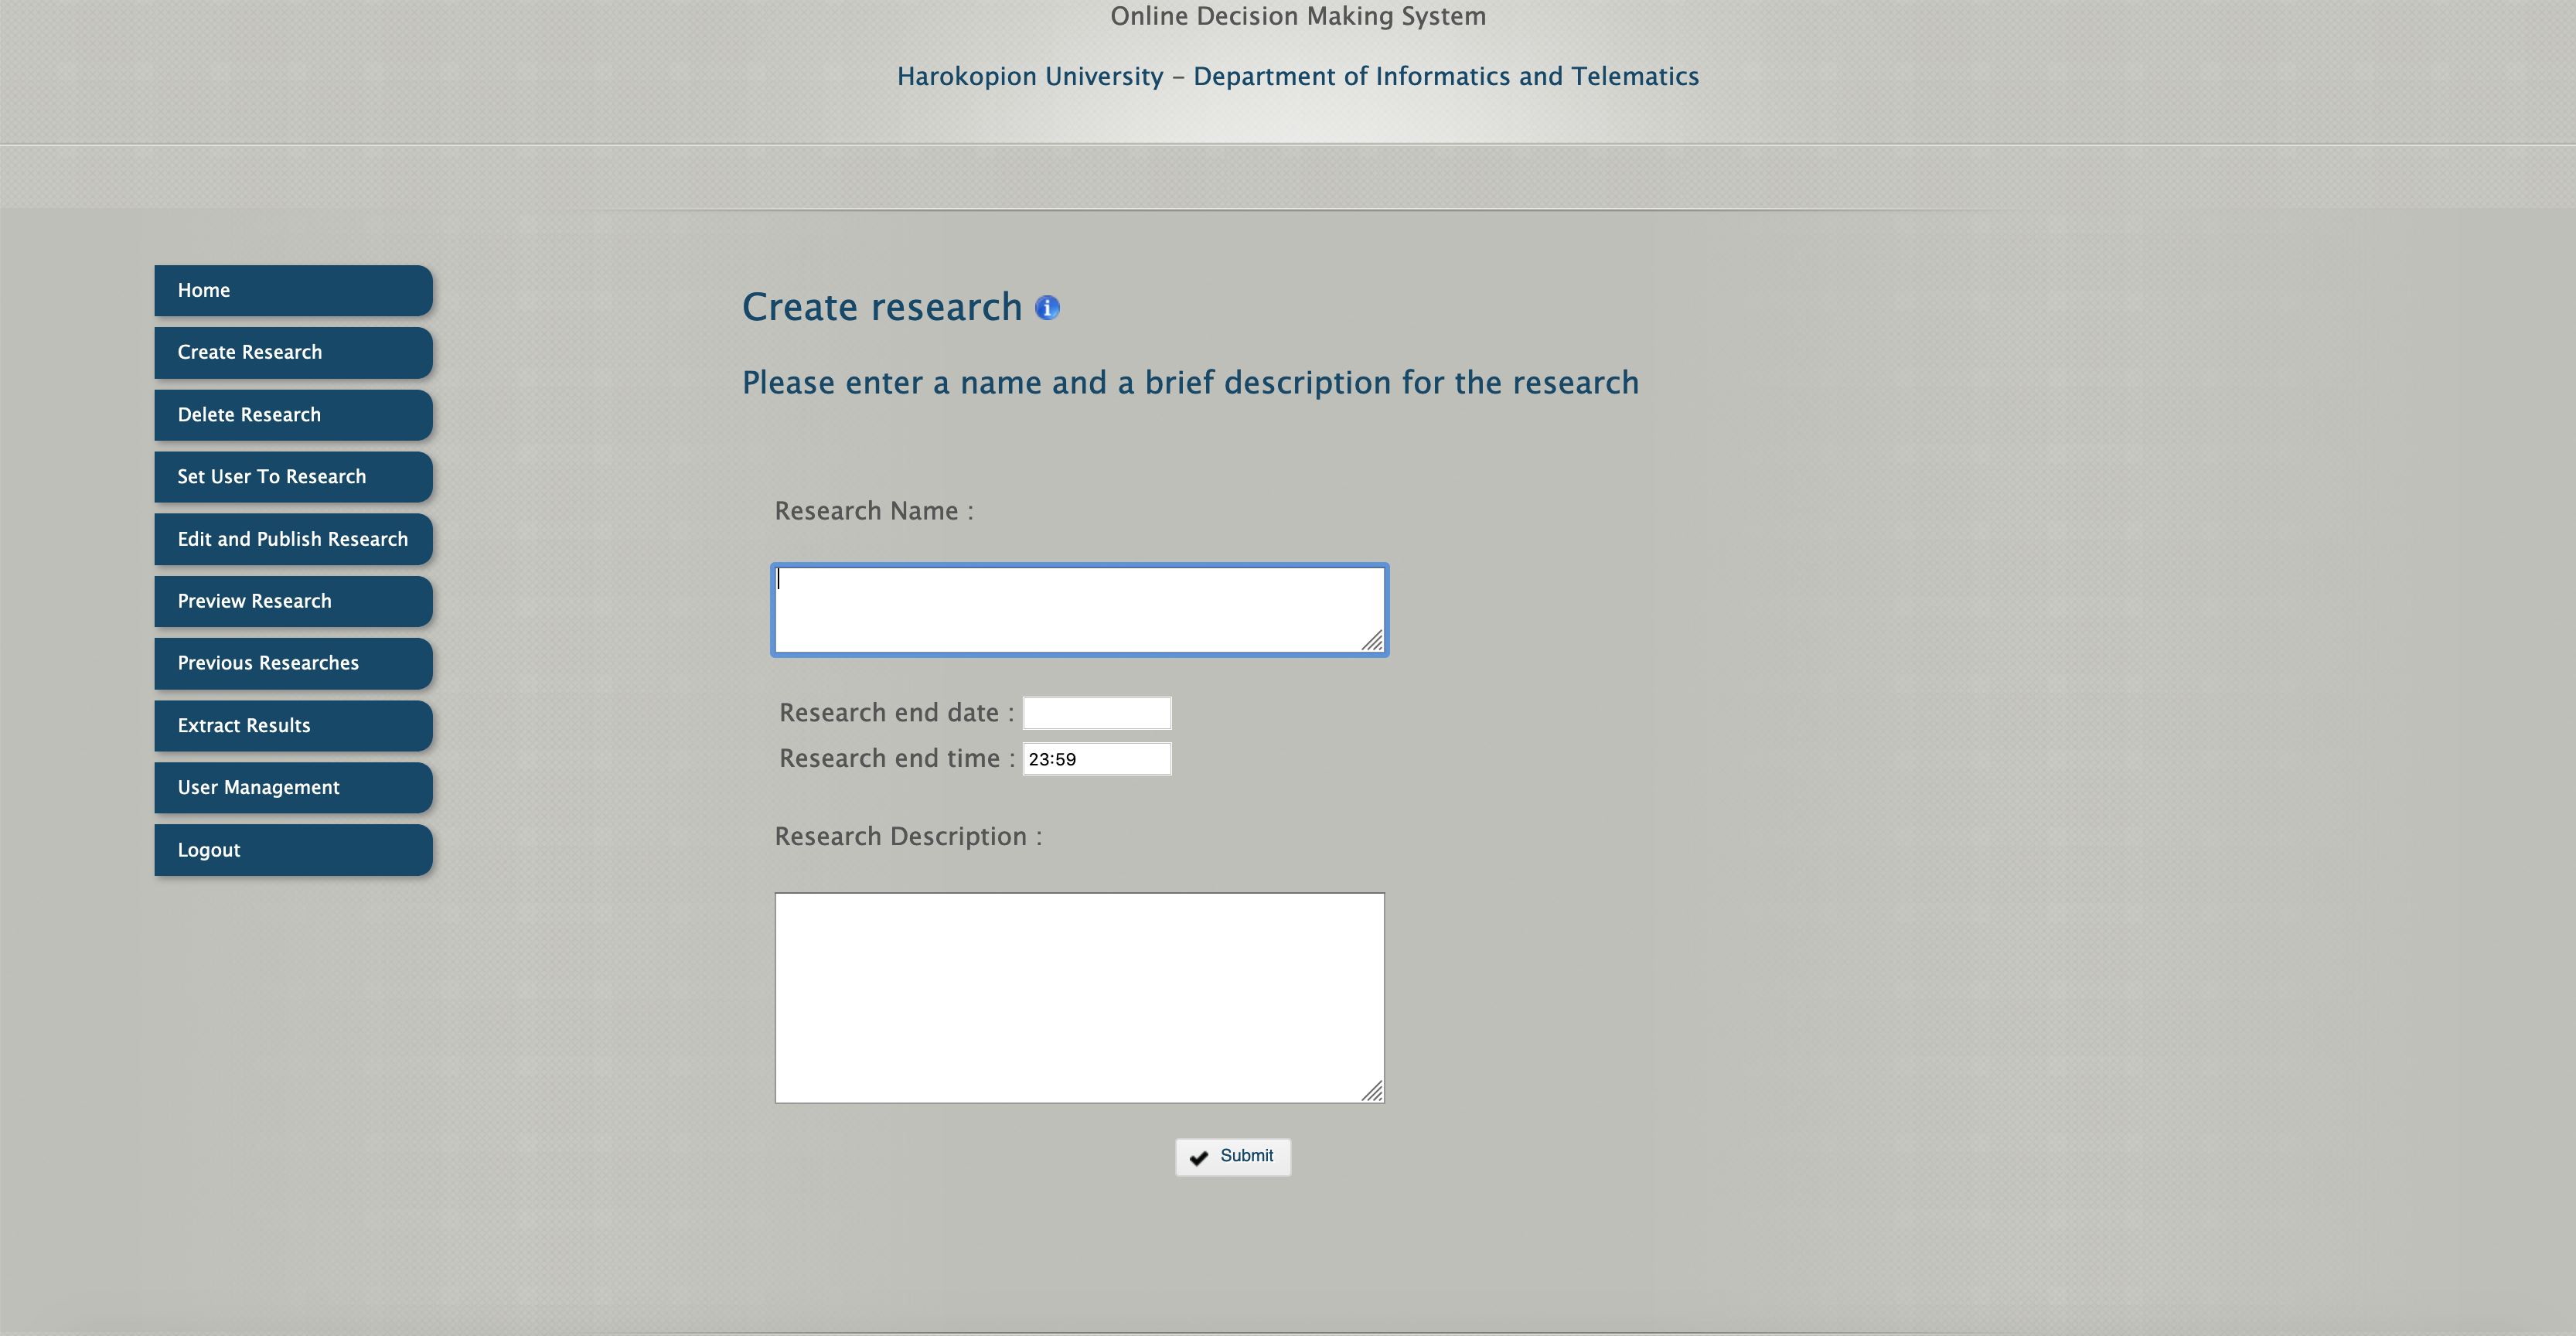
\includegraphics[scale=0.2]{create_research}
\caption{Create Survey}
\label{fig:create_survey}
\end{figure}

\begin{figure}[h!]
\centering
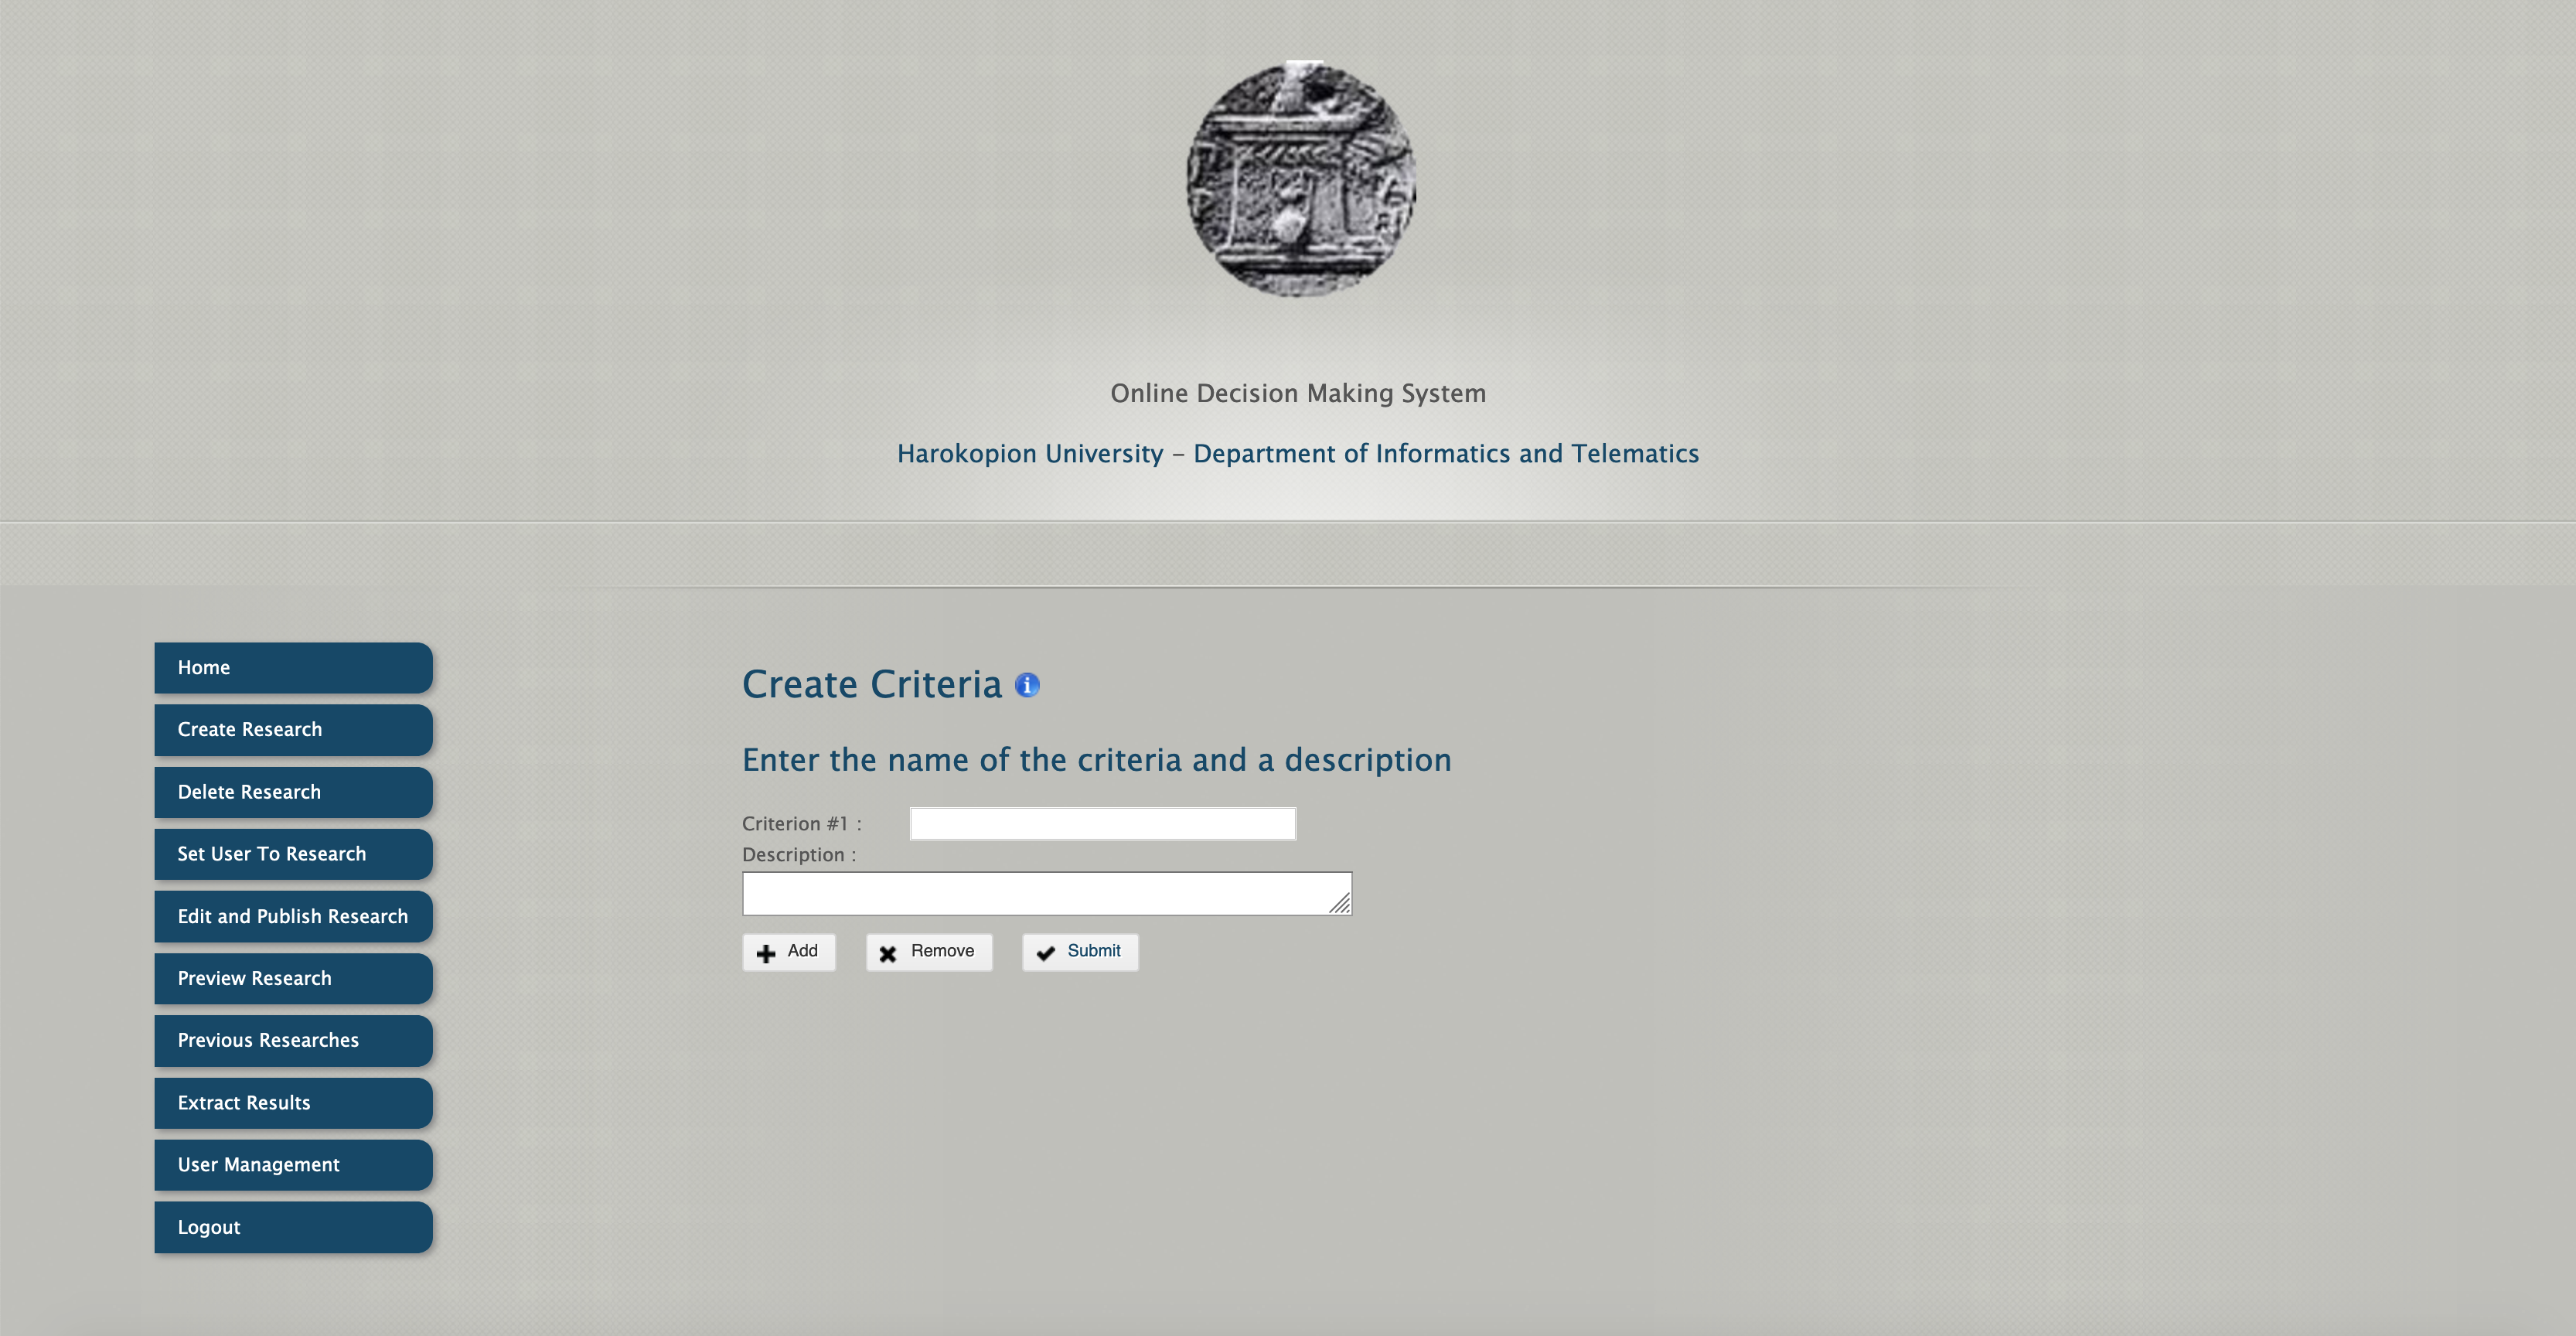
\includegraphics[scale=0.2]{create_criteria}
\caption{Create Criteria}
\label{fig:create_criteria}
\end{figure}

\begin{figure}[h!]
\centering
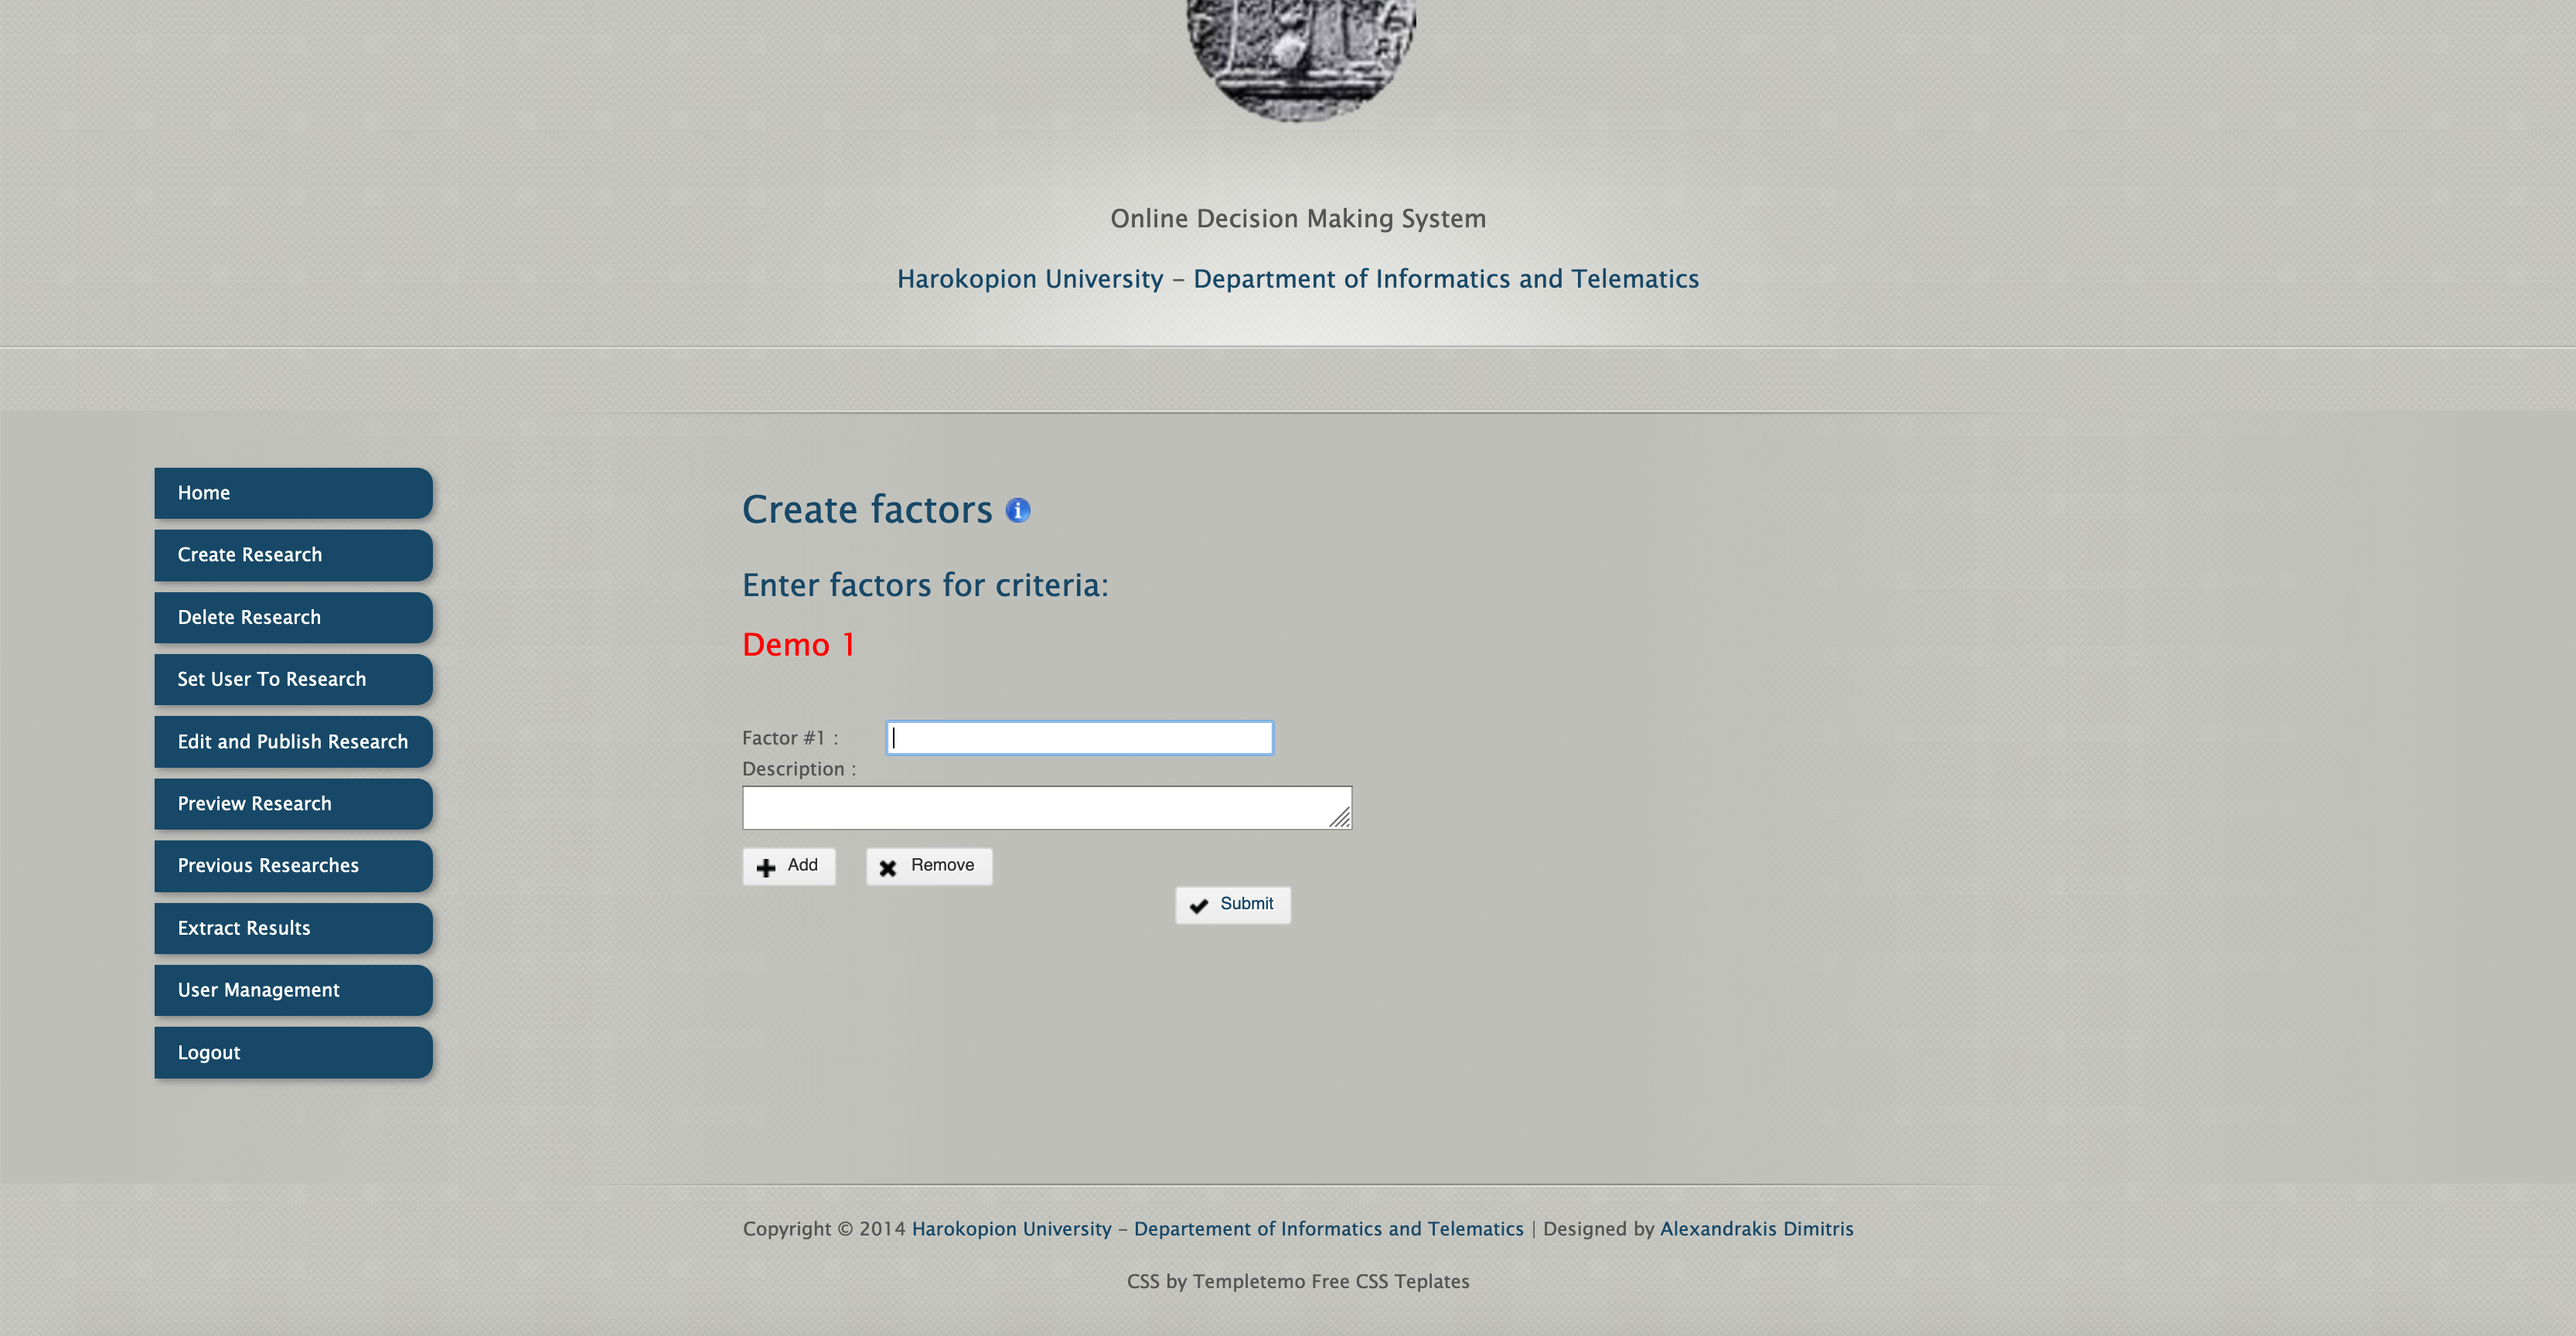
\includegraphics[scale=0.2]{create_factors}
\caption{Create Factors}
\label{fig:create_factors}
\end{figure}

\begin{figure}[h!]
\centering

\includegraphics[scale=0.2]{create_alternatives}
\caption{Create Alternatives}
\label{fig:create_alternatives}
\end{figure}





\subsubsection*{Assigning to users and publishing for answers}

When the survey is created, the next step is to assign users to fill in the survey. This can be achieved by pressing the Set User to Research button in the sidebar.





\begin{figure}[h!]
\centering
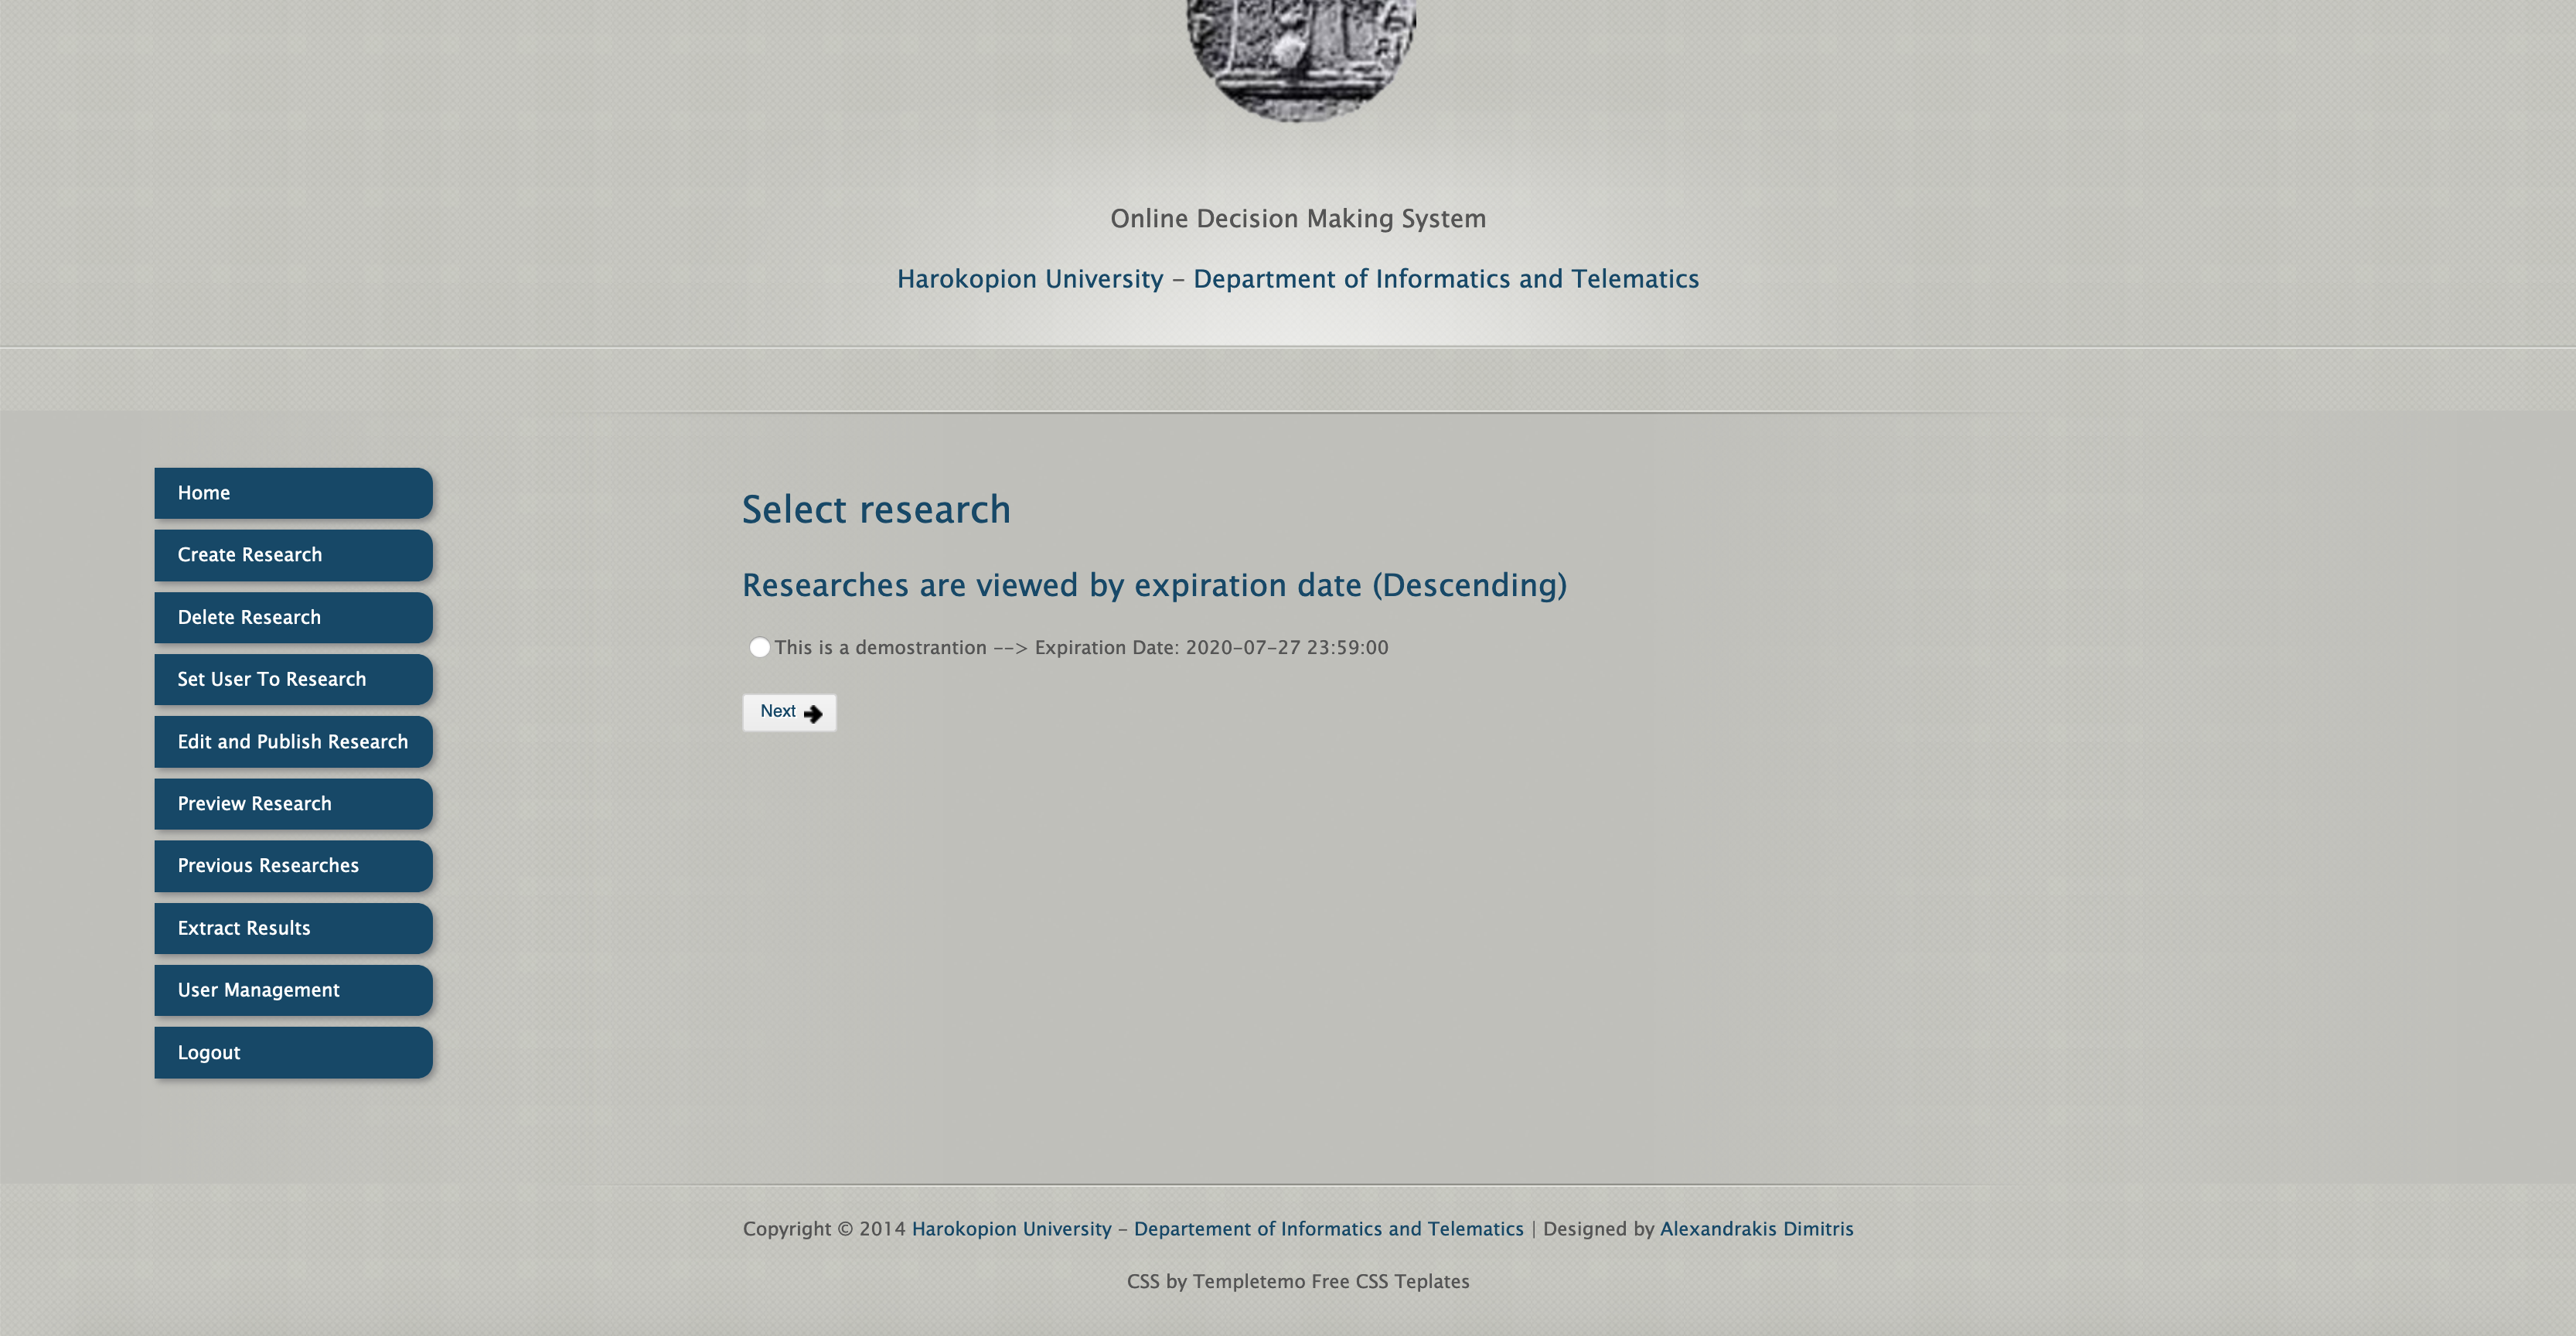
\includegraphics[scale=0.2]{assign_to_user}
\caption{Assign surveys to users}
\label{fig:assign_surveys}
\end{figure}


After that, we are ready to publish the survey. By clicking publish we are letting the system know that the survey is ready to receive answers. Once the survey is published it cannot be edited anymore. By default, a survey is considered complete when the end date, during the creation of the survey, has passed. The administrator has the possibility to complete a survey prematurely by visiting the Edit and Publish Research. When the survey is published a new button will appear that allows the administrator to complete the survey.

\begin{figure}[h!]
\centering

\includegraphics[scale=0.2]{publish}
\caption{Edit, Publish Survey}
\label{fig:edit-publish}
\end{figure}



\subsubsection*{Generating results of completed research}

When a survey is complete, either by passing the end date, or manually by the administrator, we can estimate and extract the results through the Extract Results button in the sidebar. The list of surveys that have been completed and results have not been extracted yet will be appeared.


\begin{figure}[h!]
\centering

\includegraphics[scale=0.2]{generate_results}
\caption{Generate Results}
\label{fig:generate results}
\end{figure}



Clicking on the link the calculation of the eigenvalues and eigenvectors will be performed for each user answer. Then based on the weights derived from the eigenvectors, a ranking of the alternatives is calculated and the final ranking is displayed on the screen, according to the AHP.

\begin{figure}[h!]
\centering

\includegraphics[scale=0.2]{rankings_of_alternatives}
\caption{Ranking of Alternatives}
\label{fig:ranking of alternatives}
\end{figure}


By clicking the Export button, we can get more detailed results in an Excel file.

\begin{figure}[h!]
\centering
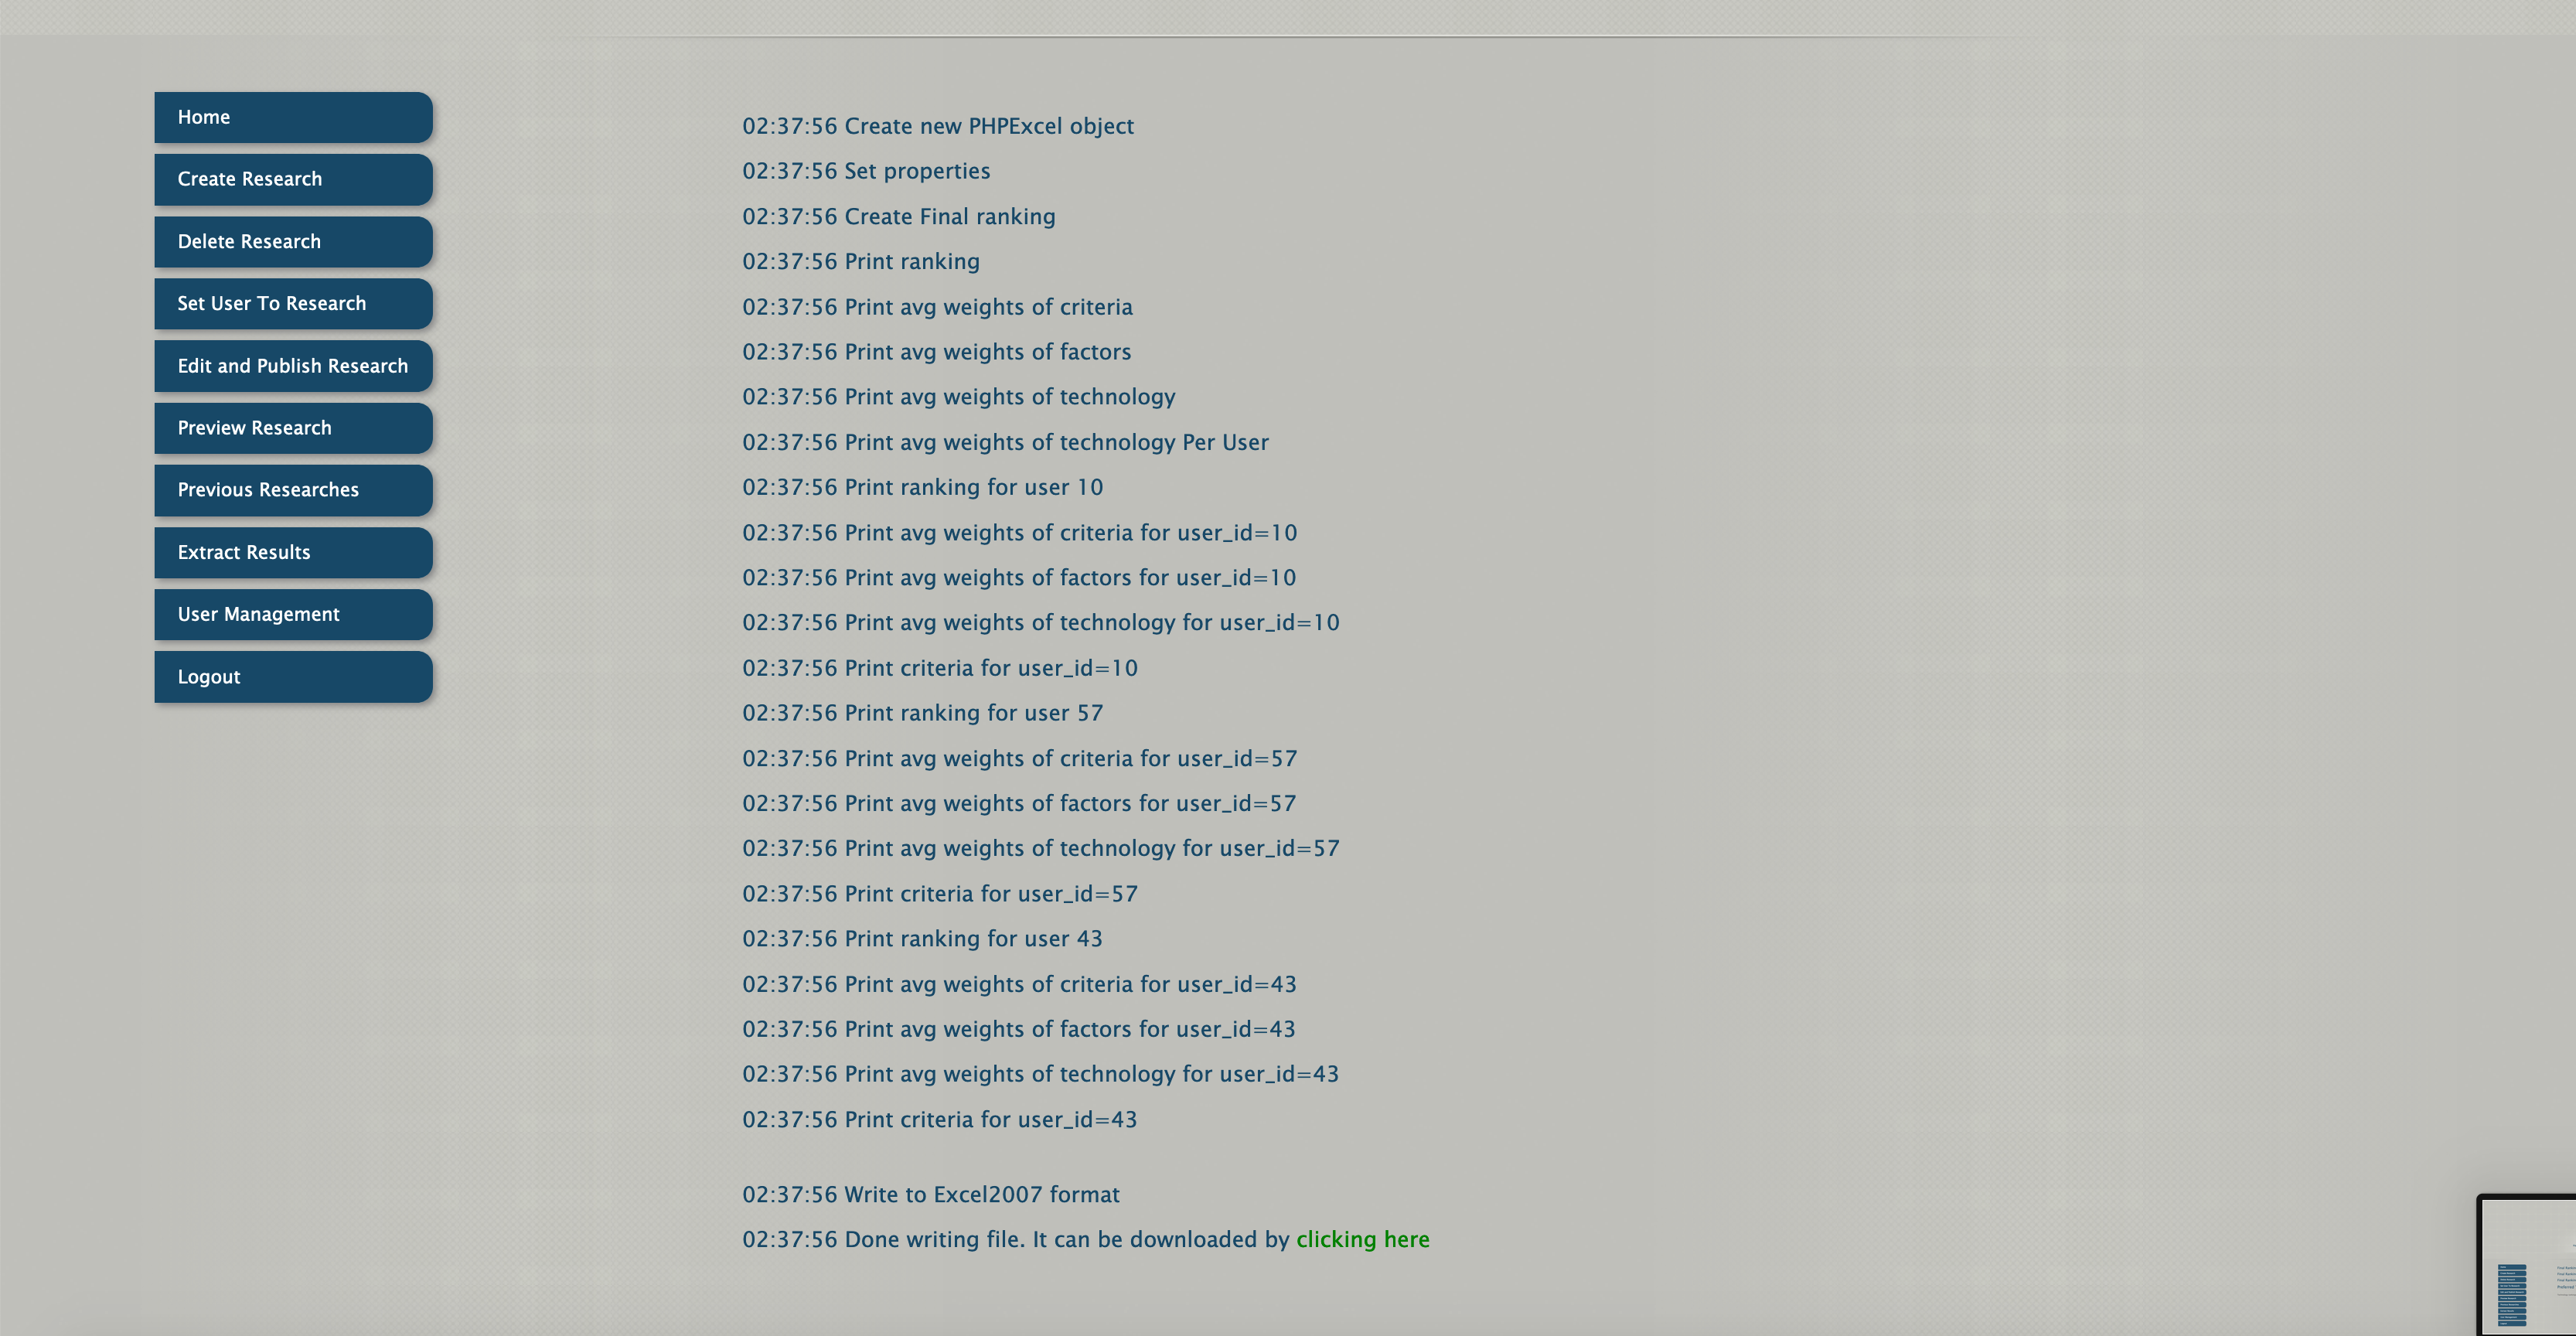
\includegraphics[scale=0.2]{extract_to_excel}
\caption{Extract results}
\label{fig:extract-to-excel}
\end{figure}

\subsection*{User}

The user is more simplified than the administrator. A user is only able to fill in an assigned survey and display previous results. For each survey a user will have instructions on how to complete his answers via a ranking system.

Example answers for an assigned survey are presented below.

\begin{figure}[h!]
\centering
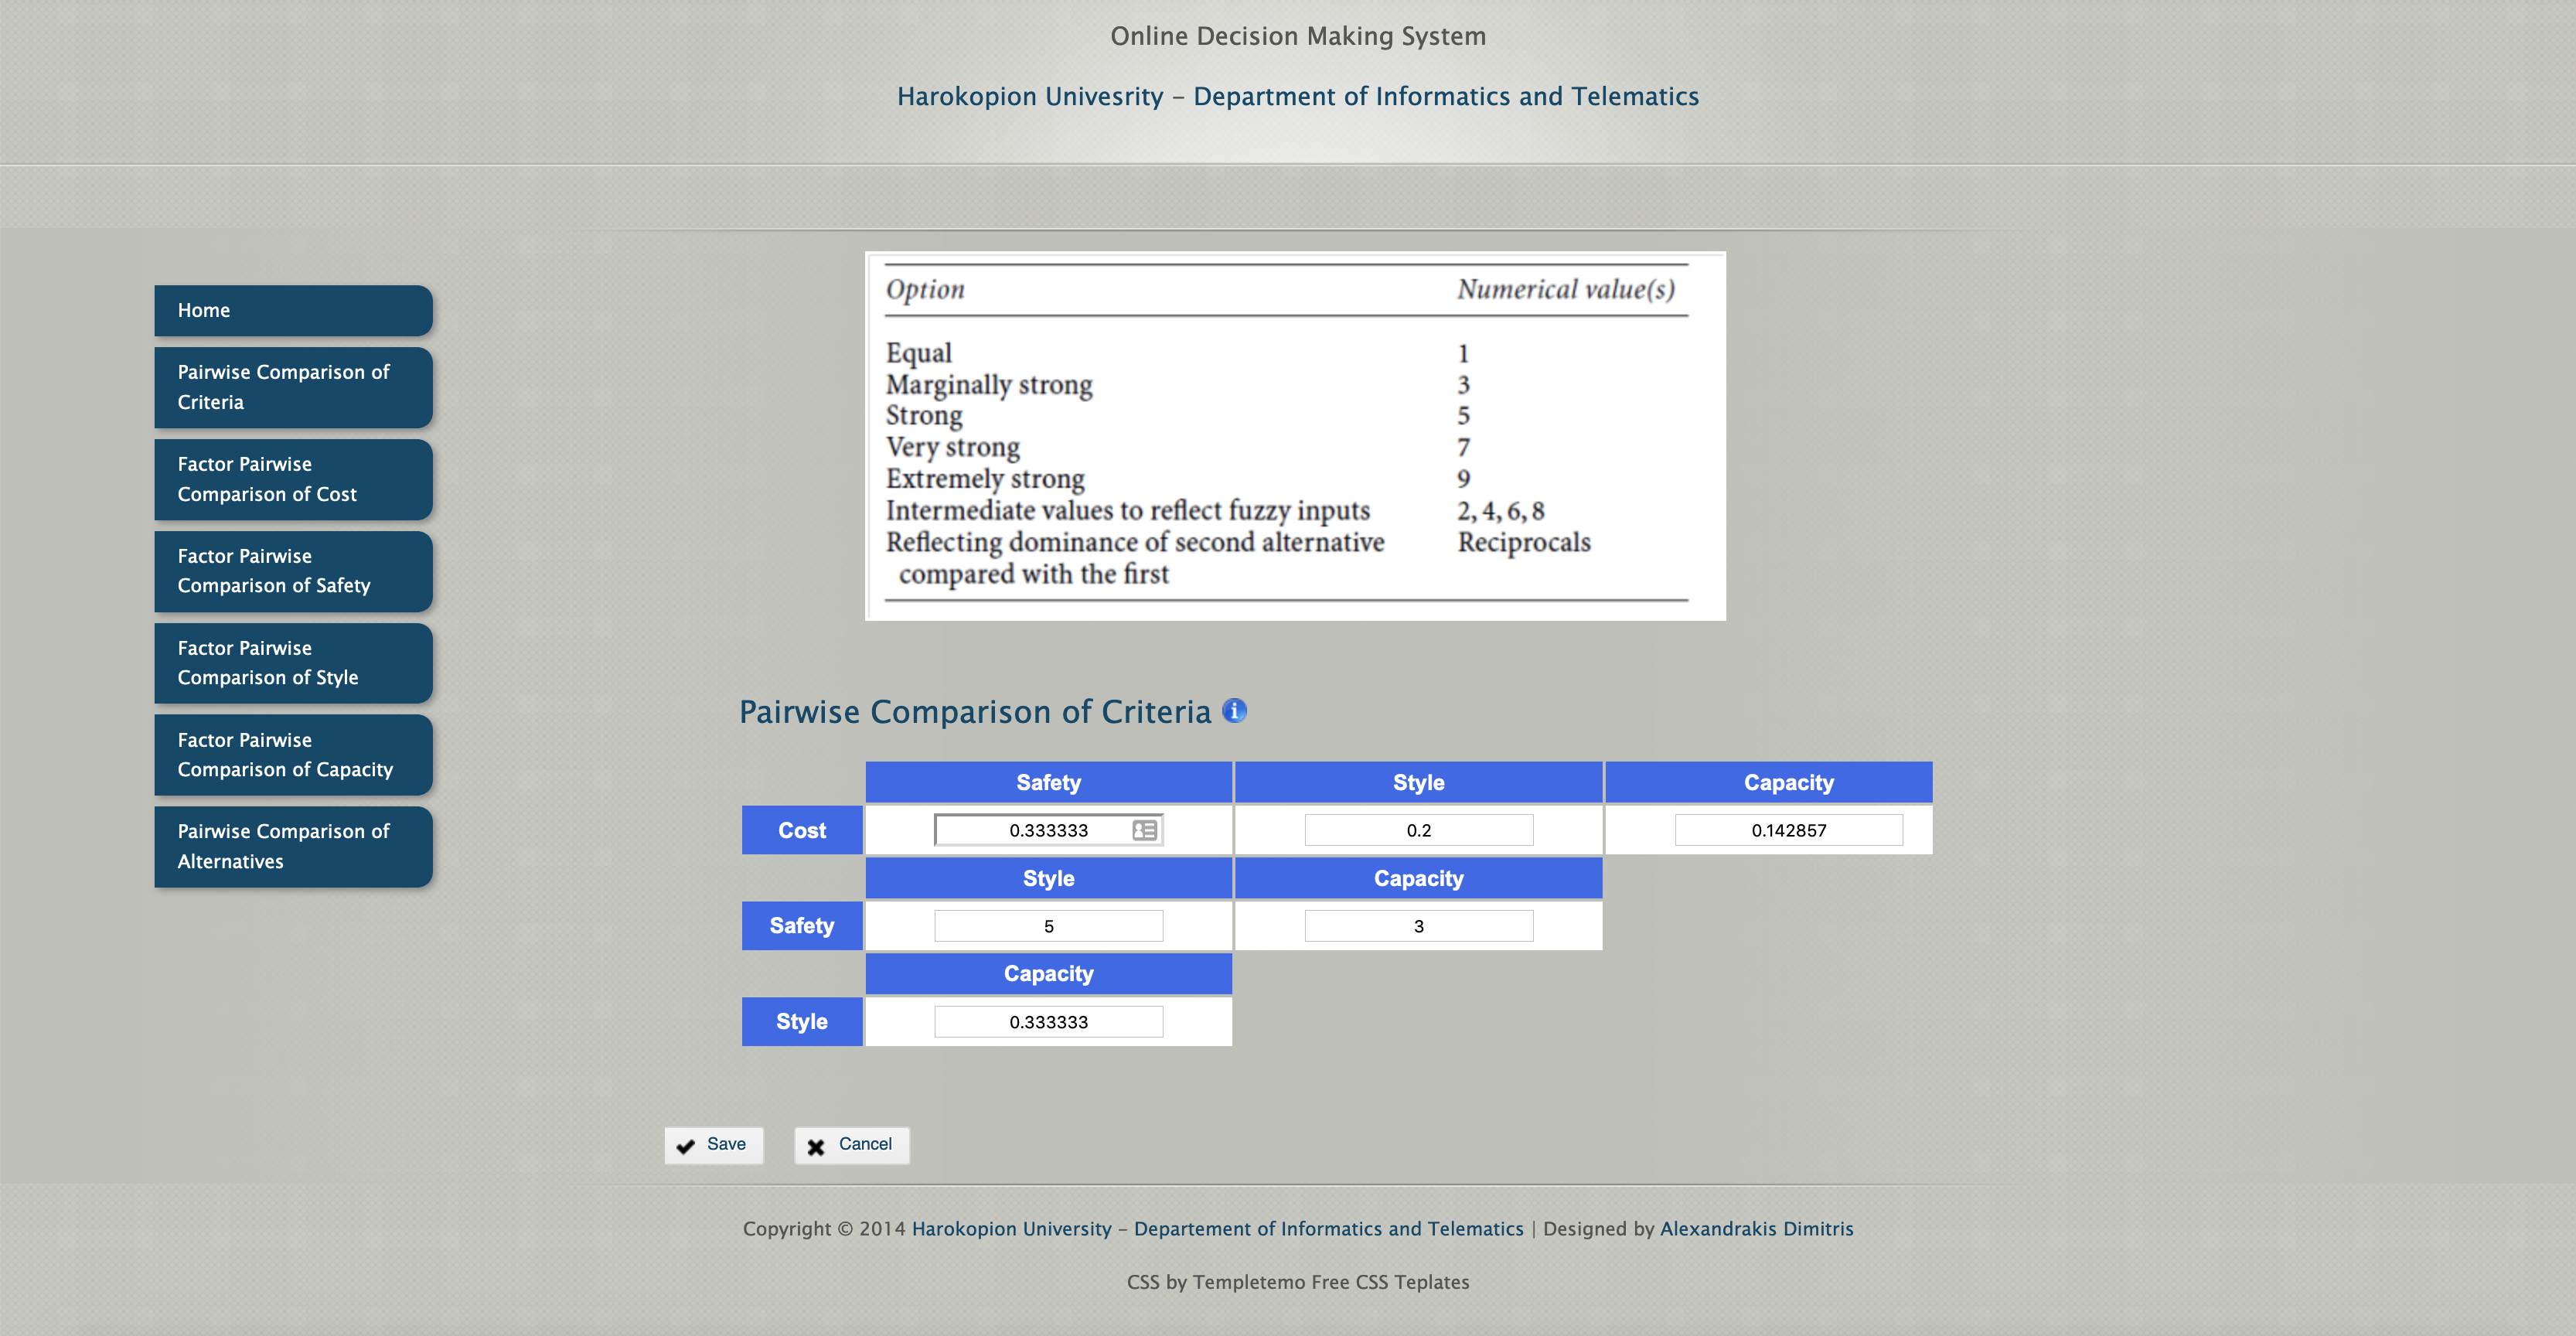
\includegraphics[scale=0.2]{user_answer}
\caption{User Answer Example 1}
\label{fig:user_answer1}
\end{figure}

\begin{figure}[h!]
\centering
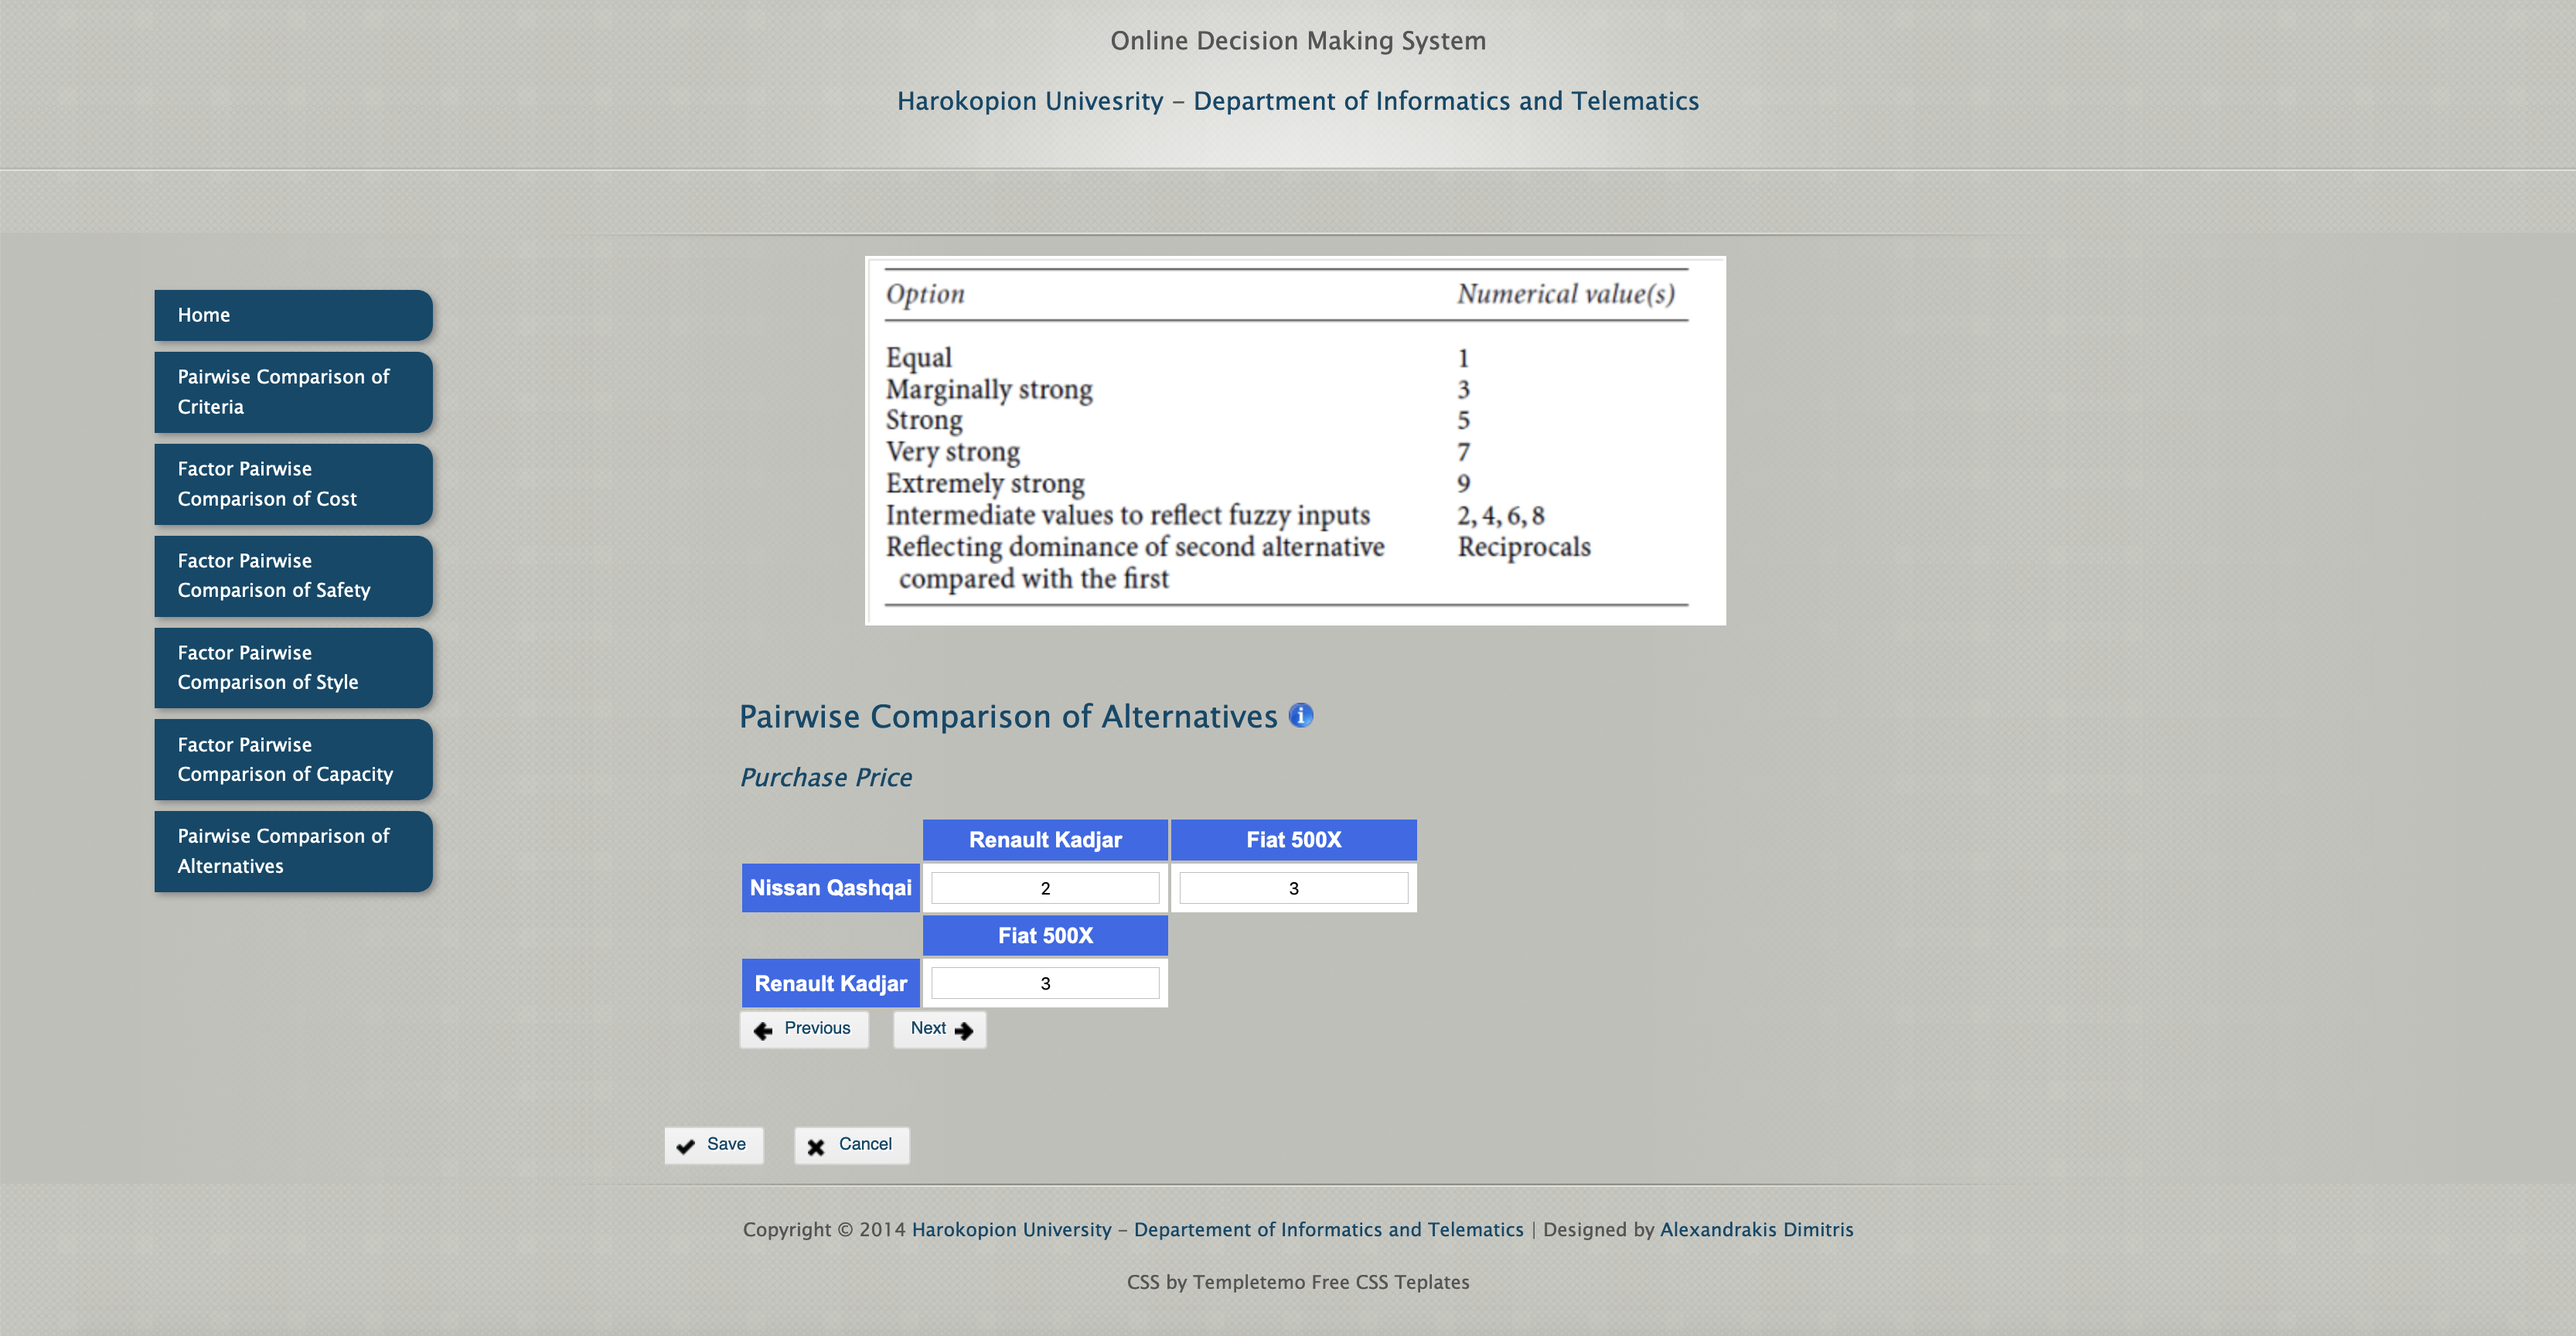
\includegraphics[scale=0.2]{user_answer2}
\caption{User Answer Example 2}
\label{fig:user_answer2}
\end{figure}

\begin{figure}[h!]
\centering
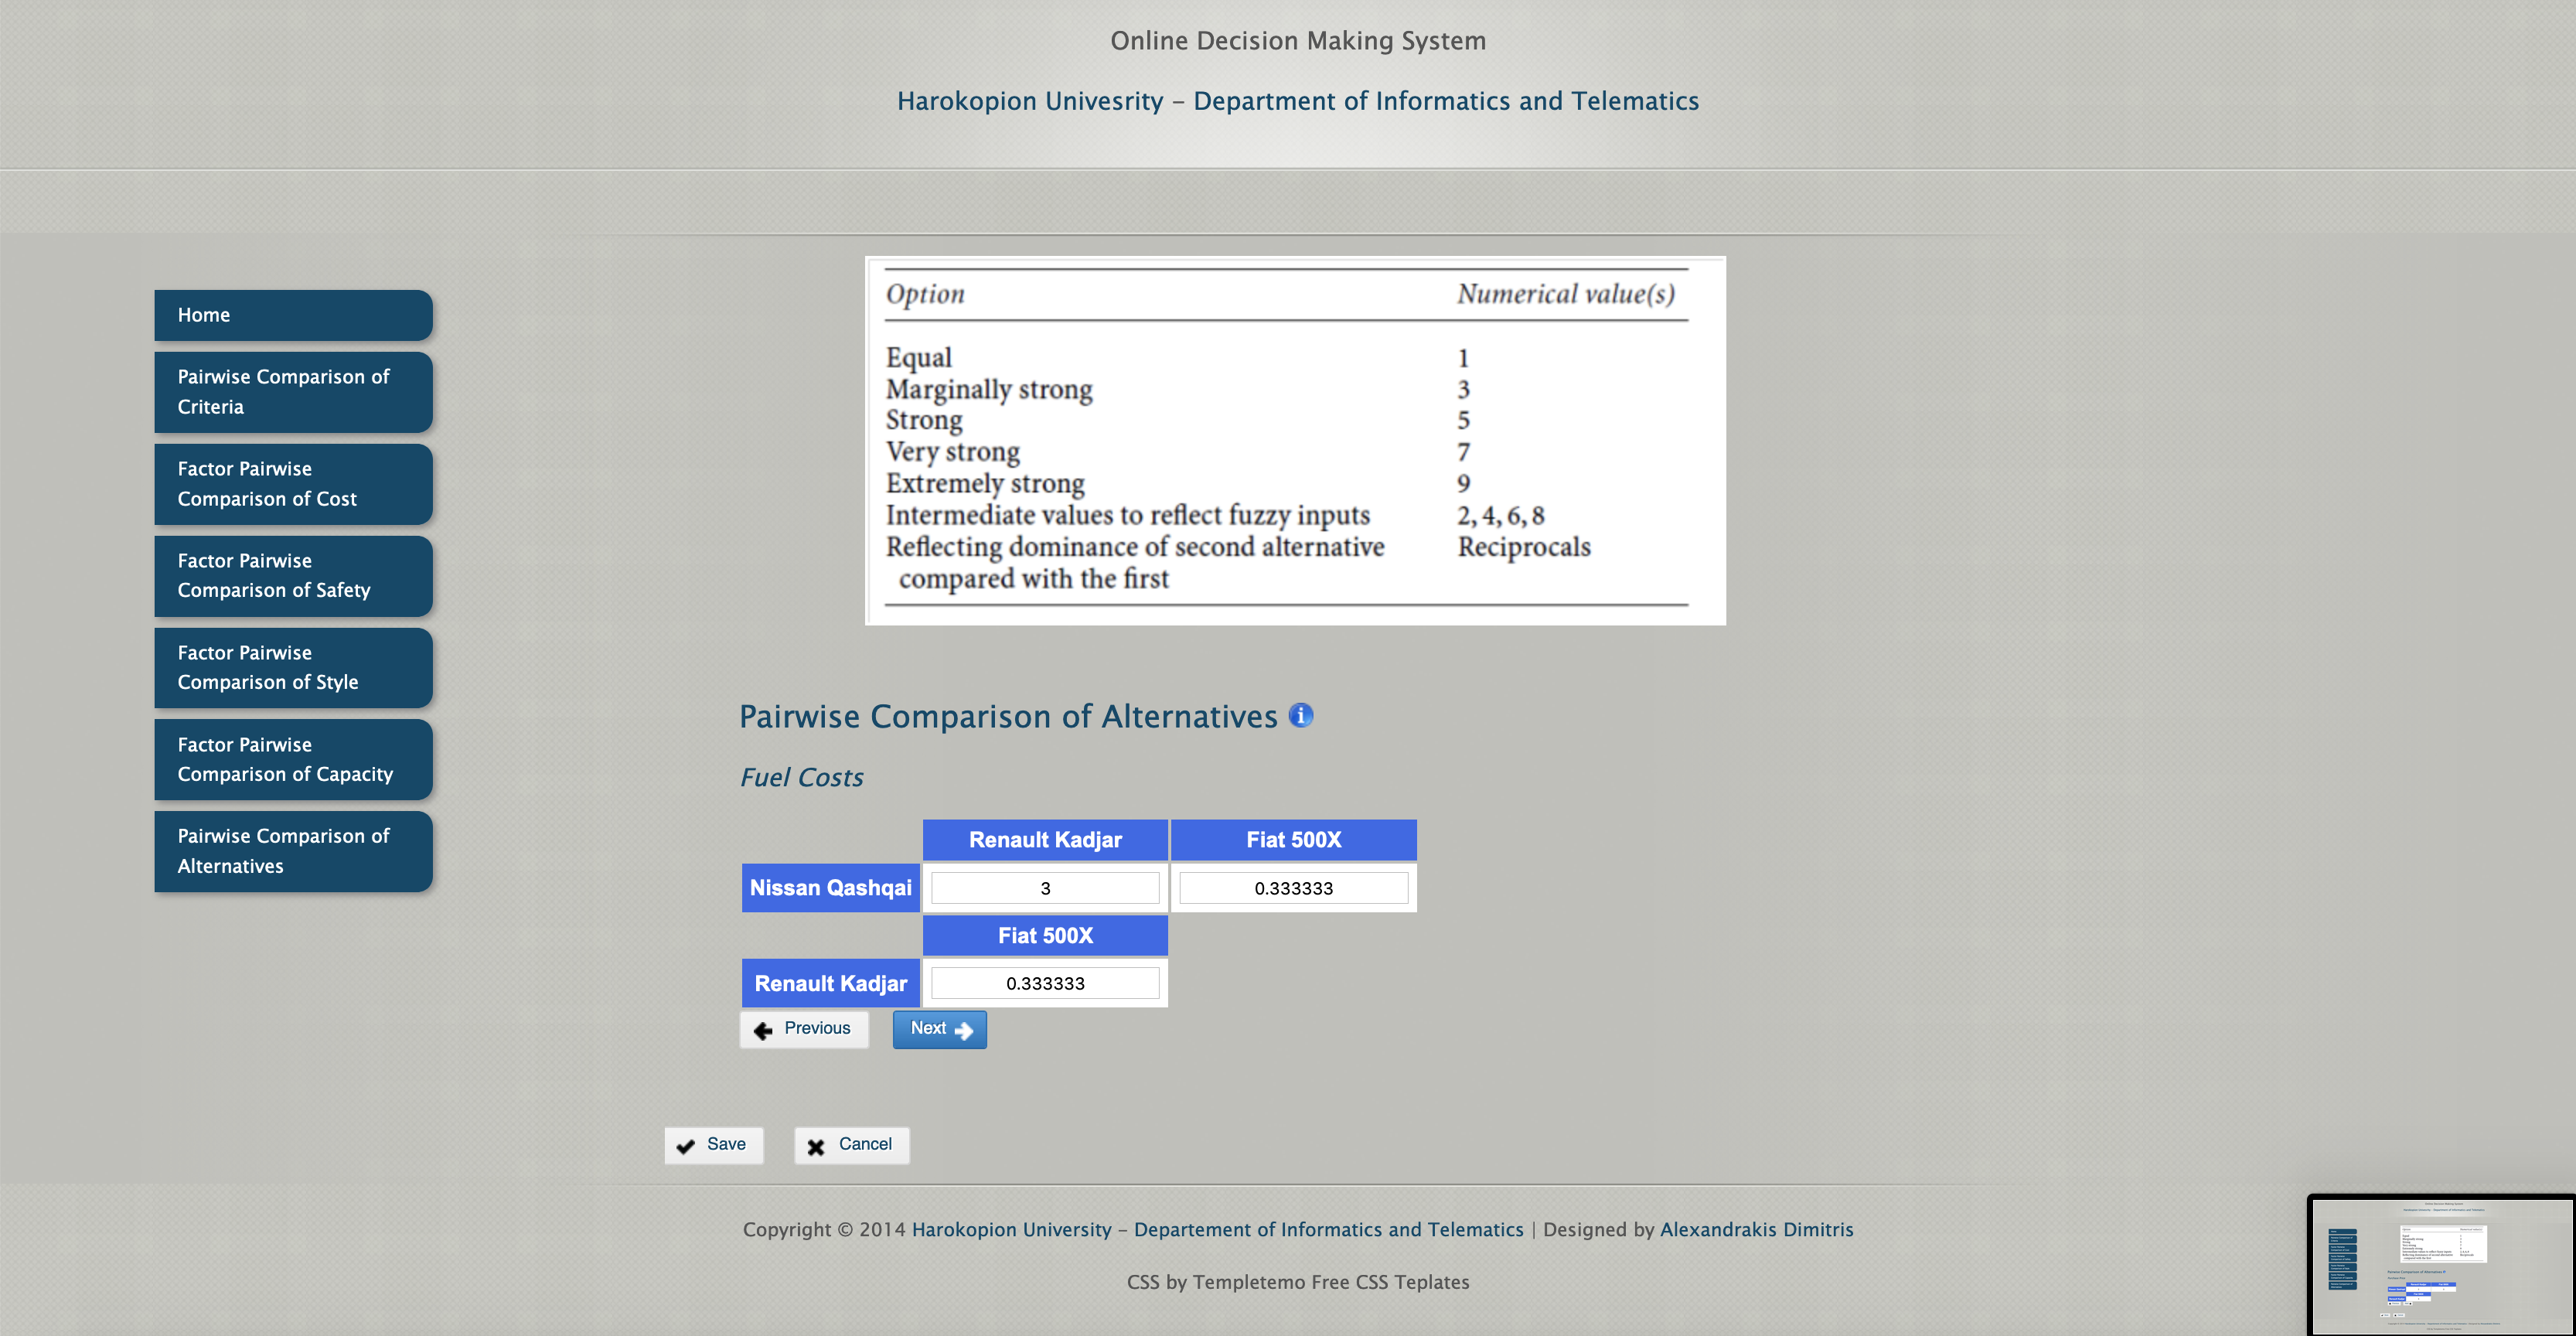
\includegraphics[scale=0.2]{user_answer3}
\caption{User Answer Example 3}
\label{fig:user_answer3}
\end{figure}


\begin{figure}[h!]
\centering
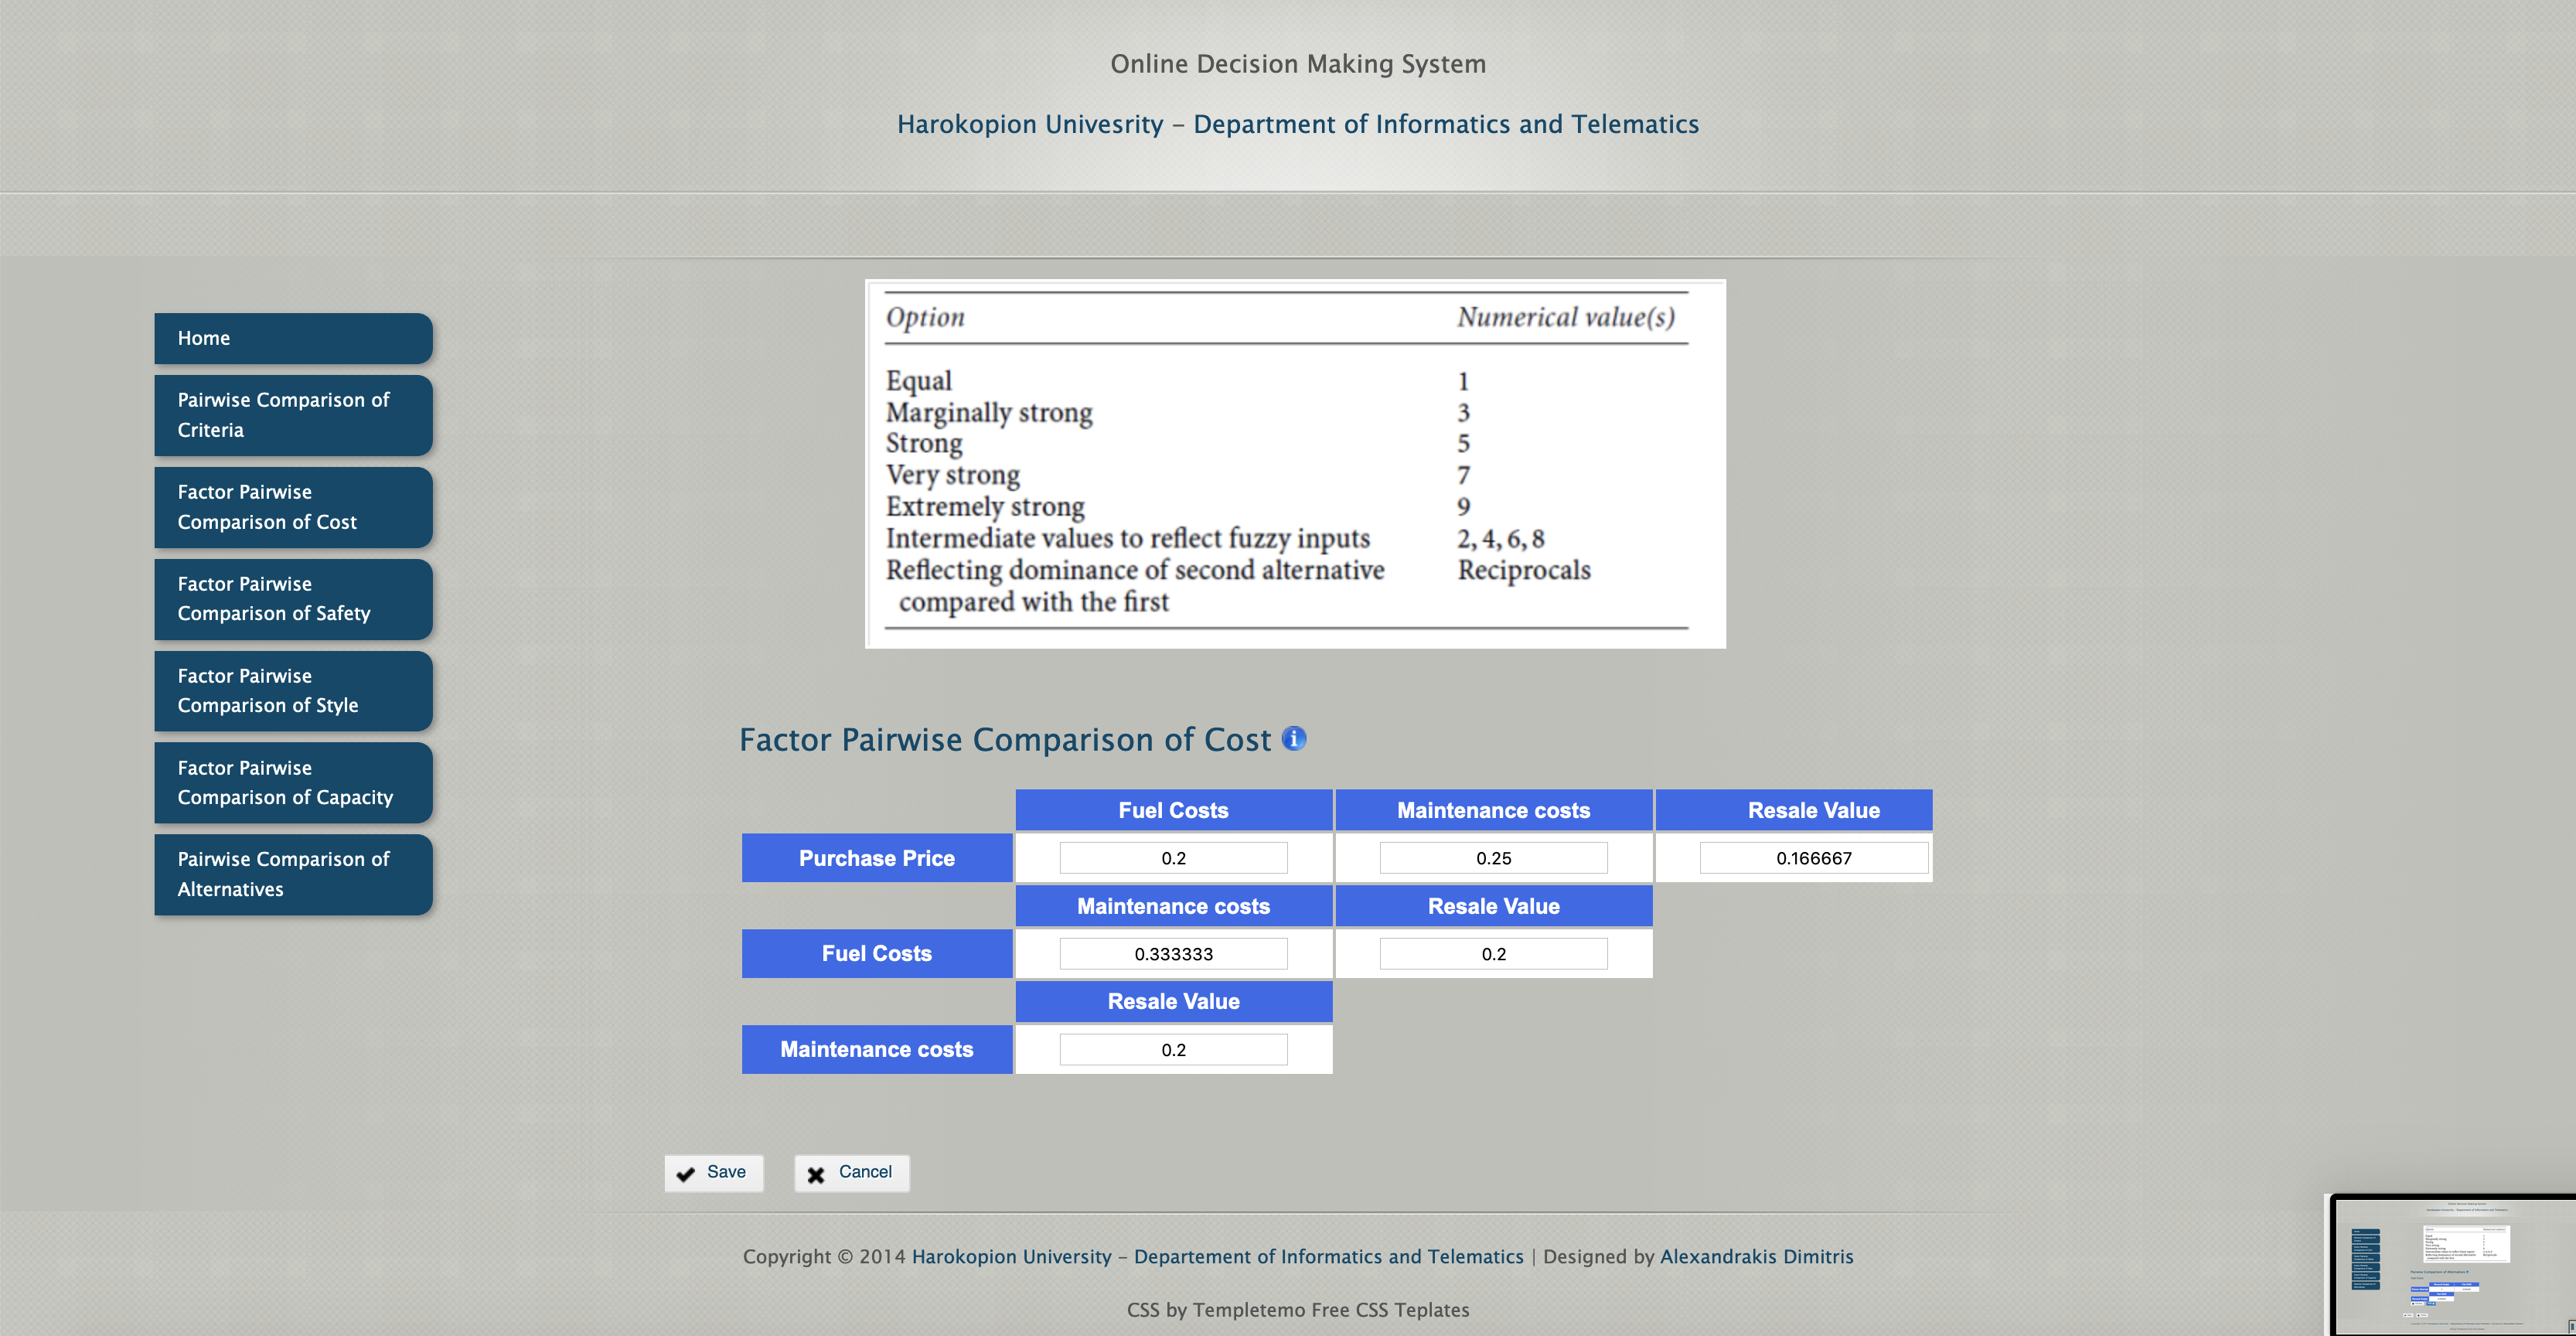
\includegraphics[scale=0.2]{user_answer4}
\caption{User Answer Example 4}
\label{fig:user_answer4}
\end{figure}


In the Completed Researches tab. The user will see a list of completed researches. By clicking the link he will be able to download the results of the research.

\begin{figure}
\centering

\includegraphics[scale=0.2]{previous_research}
\caption{Choose a research}
\label{fig:previous_research}
\end{figure}







































\bibliographystyle{plain}
\bibliography{references}
\end{document}
